\documentclass[12pt]{article}

% pacchetti
\usepackage{amsmath}
\usepackage{amscd}
%\numberwithin{equation}{subsection}
\usepackage{amssymb}
\usepackage{amsthm}
\usepackage{appendix}
\usepackage[italian]{babel} % lingua di scrittura
\usepackage{bm} % per avere simboli matematici in grassetto
\usepackage{blindtext} % per generare "Lorem ipsum dolor..." con \blindtext
\usepackage{booktabs} % per le linee nelle tabelle migliori
\usepackage{cancel} % per cancellare un testo \cancel{} per una barra verso alto a dx, mentre \xcancel{} per una croce
\usepackage{csvsimple-l3} % per convertire csv in tabelle
\usepackage{enumitem} % per fare una lista numerizzata
%\usepackage{eurosym} % per il simbolo dell'euro "€" più carino
%\usepackage{extpfeil} % per avere frecce più lunghe
% \usepackage{fontspec} % per il font calibri (NB lo spazio dopo "Calibri")
%     \setmainfont{Calibri }[
%         Path = ./fonts/,
%         Extension = .ttf,
%         BoldFont = *Bold,
%         ItalicFont = *Italic,
%         UprightFont = *Regular
%     ]
\usepackage{geometry} % per la geometria del foglio
    \geometry{
        a4paper,
        total={170mm,247mm},
        left=20mm,
        top=30mm,
    }
\usepackage{graphicx} % per le immagini
\usepackage{wrapfig} % per immagini incorniciate con il testo
\usepackage{geometry}
\usepackage{indentfirst} % per indentare anche il primo paragrafo
\usepackage[hidelinks,colorlinks = true, linkcolor = Blue]{hyperref} % per gli hyperlink
\usepackage[utf8]{inputenc} % molto importante
%\usepackage{minted} % per codice (https://it.overleaf.com/learn/latex/Code_Highlighting_with_minted)
\usepackage{multicol} % per avere parti del testo a più colonne
    % \setlength{\columnseprule}{0.5pt} % Separator ruler width
    % \def\columnseprulecolor{\color{gray}} % Separator ruler colour
\usepackage{multirow} % per avere più righe o colonne unite nelle tabelle
\usepackage{siunitx} % per avere i font per unità internazionali (per esempio microsecondi usare in TEXT MODE "\unit{\micro\second}")
\usepackage{url}
\usepackage[svgnames]{xcolor}

% \usepackage{setspace} % per l'interlinea
% \usepackage[skip=0pt plus2pt, indent = 30pt]{parskip} % spaziatura tra paragrafi
%     %\setlength{\parindent}{15pt}
%     \singlespacing %\doublespacing e \onehalfspacing

\usepackage{tikz}
\usepackage[most]{tcolorbox} % per i testi con la cornice (più info su https://ctan.mirror.garr.it/mirrors/ctan/macros/latex/contrib/tcolorbox/tcolorbox.pdf)
    %\tcbuselibrary{skins}
    \newtcolorbox[]{mvpeqbox}[1]{ % [1] sta per "1 variab. di input
                    title = \textit{{#1}}, % {#1} è la variabile inserita obbligatoria
                    sharp corners, % round corners
                    %colframe = red!50!white, % colore cornice
                    %colback = red!50!white, % colore sfondo
                    boxrule = -0.5pt, % spessore cornice
                    %opacityframe = 0, % opacità cornice
                    %opacityback = 1, % opacità sfondo
                    colbacktitle = white!87!black, % colore sfondo del titolo
                    coltitle = blue, % colore font titolo
                    ams align, % per avere l'ambiente di align
    } % custom tcolorbox per i blocchi di normali equazioni
    \newtcolorbox[]{eqbox}[1]{ % [1] sta per "1 variab. di input
                    title = #1, % #1 è la variabile inserita
                    sharp corners, % round corners
                    colframe = white!95!black, % colore cornice
                    colback = white, % colore sfondo
                    boxrule = 00.75pt, % spessore cornice
                    %opacityframe = 0, % opacità cornice
                    %opacityback = 1, % opacità sfondo
                    colbacktitle = white!95!black, % colore sfondo del titolo
                    coltitle = black, % colore font titolo
                    ams align, % per avere l'ambiente di align
    } % custom tcolorbox per i blocchi di equazione IMPORTANTI
    \newtcolorbox[]{mvvpeqbox}[1]{
                    title = \textit{{#1}},
                    sharp corners, % round corners
                    boxrule = -0.5pt, % spessore cornice
                    colbacktitle = white!87!black, % colore sfondo del titolo
                    coltitle = blue, % colore font titolo
                    ams align,
    } % custom tcolorbox per i blocchi di normali equazioni
\usepackage{circuitikz} % per realizzare circuiti con tikz(fa l'updload automatico del pacchetto tikz) 
%   \usetikzlibrary{patterns,plotmarks} % per usare root con tikz

\usepackage{fancyhdr} % per i headings e footers
    \pagestyle{fancy}
    \fancyhf{}
    \rhead{\textsc{Giovanni Boccia}, \textsc{Leandro Ye}}
    \lhead{Misura della caratteristica di uscita di un BJT}
    \fancyfoot[c]{\thepage}

\usepackage{caption} % per avere didascalie migliori
    \captionsetup{width=0.9\textwidth} % settings di caption
    \DeclareCaptionFormat{custom} % un altro setting di caption
    {
        #1#2\textit{\small #3}
    }
    \captionsetup{format=custom}
\usepackage{soul} % per highlight migliore (\hl{} per sottolineare)
\usepackage{subcaption} % per più immagini in un unico ambiente figure alla volta

%//////////////////////////////////////////////////////
%/////////////(ri)definizioni varie////////////////////
%//////////////////////////////////////////////////////

% Per settare una dilatazione delle altezze delle righe
\renewcommand{\arraystretch}{1.15}

% Per Re ed Im molto più belli (secondo me)
\renewcommand{\Re}{\operatorname{Re}}
\renewcommand{\Im}{\operatorname{Im}}

% Per scrivere velocemente le derivate parziali
% comando: \pd{#1}{#2}
\newcommand{\pd}[2]{\dfrac{\partial #1}{\partial #2}}

% Per scrivere velocemente tra i capolari ("< >")
% comando: \lrangle{#1}
\newcommand{\lrangle}[1]{\langle #1 \rangle}

% Per scrivere i vari ±1/2 etc (SOLO NELLE EQUAZIONI)
\newcommand{\pmoh}{{\pm\frac{1}{2}}} % ±1/2
\newcommand{\mpoh}{{\mp\frac{1}{2}}} % ∓1/2
\newcommand{\poh}{{+\frac{1}{2}}} % +1/2
\newcommand{\moh}{{-\frac{1}{2}}} % -1/2

% \definecolor{bg}{rgb}{0.95,0.95,0.95}
% \definecolor{green}{rgb}{0,.66,0}
% \definecolor{white}{rgb}{1, 1, 1}

\begin{document}

% frontespizio
%\thispagestyle{plain} % per ignorare per questa pagina le impostazioni fancy
\thispagestyle{empty} % per disattivare per questa pagina le impostazioni fancy e anche il numero della pagina

\begin{figure}[h]
    \centering
    \includegraphics[width=0.5\textwidth]{image/logo.png}
    \label{Logo}
\end{figure}

\vspace{0.5cm}

\begin{center}
{\large \textsc{PROVA 2}}
\end{center}

\section*{\centering \Huge \bf Misura della caratteristica di uscita \\di un BJT PNP in configurazione \\ a emettitore comune}

\vspace{3cm}

\begin{center}
{\large Realizzato da} \\
\vspace{2cm}

\begin{multicols}{2}
    \Large\textsc{Giovanni Boccia}\\ 000 1032154\\
    \Large\textsc{Leandro Ye}\\ 000 1050281\\
\end{multicols}
 
\end{center}

\vspace{3cm}

\begin{center}
{\large Tavolo 15, turno 1}\\
\vspace{1cm}
{\large 30 novembre 2023}
\end{center}

\newpage

\section*{Abstract}
Lo scopo dell’esperienza è stato quello di misurare la caratteristica I-V di un transistor BJT PNP a emettitore comune. In particolare, abbiamo acquisito le misure della tensione tra collettore ed emettitore e della corrente di collettore per due diversi valori della corrente di base, ossia $I_{B_1} = -50$ \si{\micro A} e $I_{B_2} = -100$ \si{\micro A}.\\
Mediante un fit sono stati poi calcolati la tensione di Early $V_a$ e la resistenza di uscita $R_L$ per ogni curva, da cui è stato possibile ricavare il guadagno $\beta$ e la conduttanza $g$. Per quanto riguarda i valori dei parametri trovati per $I_{B_1}$, abbiamo ottenuto $V_{a_1} = (24 \pm 5)$ \si{V} e $R_{L_1} = (3.0 \pm 0.5)$ \si{k\ohm} da cui abbiamo poi ricavato la conduttanza $g_1 = (0.33 \pm 0.06)$ \si{\milli\siemens}. Per la corrente di base $I_{B_2}$ invece abbiamo trovato $V_{a_2} = (23 \pm 4)$ \si{V} e $R_{L_2} = (1.6\pm 0.3)$ \si{k\ohm} da cui abbiamo poi ricavato $g_2 = (0.63 \pm 0.12)$ \si{\milli\siemens}. È stato infine possibile calcolare il guadagno di corrente $\beta = (1.3 \pm 1.1) \cdot 10^{2}$, a prova del fatto che il BJT in questa configurazione si comporta come un amplificatore di corrente.

\section{Introduzione}
Il transistor BJT è un dispositivo realizzato con un cristallo semiconduttore composto da tre regioni: due drogate di tipo n e una drogata di tipo p o due regioni drogate di tipo p e una di tipo n. Le tre regioni sono dette emettitore (E), base (B) e collettore (C). In particolare, lo scopo dell’esperienza è stato quello di misurare la caratteristica di un BJT PNP ad emettitore comune, ossia una configurazione in cui l’emettitore è collegato direttamente a massa. In questa configurazione il transistor si comporta come amplificatore di corrente e tensione. 
L’andamento delle correnti all’interno di un transistor è descritto dalle relazioni di Embers-Moll:
\begin{equation}\label{eq:ES_eqs}
    \begin{cases}
    I_E = -I_{ES}\Biggl(e^\dfrac{V_{BE}}{\eta V_T} - 1\Biggl) + \alpha_R I_{CS} \Biggl(e^\dfrac{V_{BC}}{\eta V_T} - 1\Biggl)\\
    I_C = -I_{CS}\Biggl(e^\dfrac{V_{BC}}{\eta V_T} - 1\Biggl) + \alpha_F I_{ES} \Biggl(e^\dfrac{V_{BE}}{\eta V_T} - 1\Biggl)\\
    \end{cases}
\end{equation}
Dove $I_E$ è la corrente d'emettitore e $I_C$ è la corrente di collettore, mentre $V_{BC}$ è la tensione tra base e collettore e $V_{BE}$ è la tensione tra base ed emettitore. Infine, $I_{ES}$ e $I_{CS}$ sono le correnti di saturazione dell’emettitore e del collettore rispettivamente.\\
Noi siamo interessati al funzionamento del BJT in regione attiva, ossia quando la giunzione base-emettitore è polarizzata direttamente mentre la giunzione base-collettore è polarizzata inversamente, e vale la seguente relazione:
\begin{equation}\label{eq:ES_active}
    I_C\ (V_{BE}) = \alpha_F I_{ES}\Biggl(e^\dfrac{V_{BE}}{\eta V_T} - 1\Biggl)
\end{equation}
Si noti che in questa configurazione i valori di $I_C$ e $V_{BE}$ sono negativi. L’\autoref{eq:ES_active} prevede una rapida crescita, seguita da un tratto pressoché costante. Quello che si nota è invece una leggera pendenza del secondo tratto, dovuta all’effetto Early, un effetto che consiste nella variazione dell’ampiezza della regione di base dovuta alla variazione della tensione della giunzione BC. Ciò tende a far crescere $I_C$ all’aumentare di $V_{CE}$. A questo punto, una volta fissata la corrente di base $I_B$, vale la seguente relazione fenomenologica:
\begin{equation*}
    V_{CE} = V_a + R_L \cdot I_C
\end{equation*}
\begin{equation}\label{eq:fit}
    I_C = \dfrac{V_{CE} - V_a}{R_L}
\end{equation}
dove $V_a$ è la tensione di Early, con valori generalmente compresi tra 10 \si{V} e 200 \si{V}, e $R_L$ è la resistenza di uscita con valori tipicamente dell'ordine di grandezza del \si{\kilo\ohm}, da cui è possibile ricavare la conduttanza $g$ sapendo che 
\begin{equation}\label{eq:conduttanza}
    g = \dfrac{1}{R_L}
\end{equation}
Inoltre, è possibile stimare il guadagno in termini di corrente per un valore fissato di $V_{CE}$ tramite 
\begin{equation}\label{eq:guadagno}
    \beta = \dfrac{\Delta I_C}{\Delta I_B} = \dfrac{I_{C_2} - I_{C_1}}{I_{B_2} - I_{B_1}}
\end{equation}


\section{Apparato sperimentale e svolgimento}
Lo scopo della prova è quello di misurare le caratteristiche I-V in uscita di un transistor BJT PNP in configurazione a emettitore comune, per due differenti valori della corrente di base.

\subsection{Materiali e strumenti}
Riportiamo adesso l'elenco dei materiali e degli strumenti utilizzati durante l’esperienza (tra parentesi il modello utilizzato):
\begin{multicols}{2}
    \begin{itemize}
         \item Generatore di tensione (\verb|ISO-TECH IPS 3303|)
        \item Potenziometro da 1\si{\kilo\ohm}
        \item Potenziometro da 100\si{\kilo\ohm}
        \item Transistor PNP al Si (\verb|BC 212|)
        \item Breadboard (\verb|K&H AD-13|)
        \item Oscilloscopio analogico (\verb|ISO-TECH ISR 622|)
        \item Multimetro digitale (\verb|Fluke 77 IV|)
        \item [\vspace{\fill}]
    \end{itemize}
\end{multicols}

\begin{table}[h]
    \centering
    \begin{tabular}{||c|c|c|c||}
        \hline\hline
        \multicolumn{4}{||c||}{\textsc{multimetro} \ \texttt{Fluke 77 IV}}\\
        \hline\hline
        fondo scala & risoluzione & prec. & digits \\\hline
        60.00 \si{\milli\ampere} & 0.01 \si{\milli\ampere} & \multirow{4}{*}{1.5\%} & \multirow{4}{*}{2}\\
        400.0 \si{\milli\ampere} & 0.1 \si{\milli\ampere} &  & \\
        6.000 \si{\ampere} & 0.001 \si{\ampere} &  & \\
        10.00 \si{\ampere} & 0.01 \si{\ampere} &  & \\
        \hline\hline
    \end{tabular}
    \caption{Specifiche tecniche del multimetro \ \emph{\texttt{Fluke 77 IV}} relative alle misurazioni di corrente in corrente continua. La colonna \emph{prec.} indica la precisione e \emph{digits} indica il numero da aggiungere all'ultima cifra significativa della misura.}
    \label{tab:multimetro}
\end{table}

\subsection{Svolgimento dell'esperienza}
\begin{figure}[htb]
    \centering
    \begin{subfigure}{.4\textwidth}
    \centering
        \begin{circuitikz}[scale = 1, every node/.style={scale=0.9}]
% \foreach \i in {0,...,6} {
%     \draw [very thin,white!80!black] (\i,0) -- (\i,6)  node [below] at (\i,0) {$\i$};
% }
% \foreach \i in {0,...,6} {
%     \draw [very thin,white!80!black] (0,\i) -- (6,\i) node [left] at (0,\i) {$\i$};
% }
\draw % cornice (in basso a sx in senso orario)
    (0,1)
    to[battery2, l_=$-5\si{\volt}$, invert] (0,6)
    -- (6,6)
    -- (6,3)
    to [pR, name=dx, mirror, wiper pos=0.2] (6,1)
    -- (0,1)
;
\draw % potenziometro di sx (dal basso)
    (1.5,1) node[circ]{}
    -- (1.5,3.5)
    to[pR, l=1\si{\kilo\ohm}, name=sx, mirror, wiper pos=0.7] (1.5,6)
    node[circ]{}
;
\draw % bjt (dal basso)
    (3,1) node[circ]{}
    -- (3,3)
    node[pnp, anchor=E, xscale=-1, yscale=-1, tr circle] (bjt) {}
    (bjt.collector) |- (sx.wiper) % da C a sx
;
\draw % amperometro (dal bjt in alto)
    (bjt.base)
    -| (4.75,3.6)
    to[smeter, t=A, l=$I_B$] (4.75,2.5)
    |- (dx.wiper)
;
\draw (dx) node[left=3pt] {100\si{k\ohm}};
\node [circ] at (bjt.circle C){};
\draw (bjt.circle C) node[above left] {$C$};
\node [circ] at (bjt.circle E){};
\draw (bjt.circle E) node[below left] {$E$};
\node [circ] at (bjt.circle base){};
\draw (bjt.circle base) node[above right] {$B$};
\end{circuitikz}
        \caption{Schema del circuito realizzato per il regolamento della corrente di base al punto \emph B.}
        \label{fig:circ_1}
    \end{subfigure}
     \hspace{1cm}
    \begin{subfigure}{.4\textwidth}
        \centering
        \begin{circuitikz}[scale = 1, every node/.style={scale=0.9}]
% \foreach \i in {0,...,6} {
%     \draw [very thin,white!80!black] (\i,0) -- (\i,6)  node [below] at (\i,0) {$\i$};
% }
% \foreach \i in {0,...,6} {
%     \draw [very thin,white!80!black] (0,\i) -- (6,\i) node [left] at (0,\i) {$\i$};
% }
\draw % cornice (in basso a sx in senso orario)
    (0,1)
    to[battery2, l_=$-5\si{\volt}$, invert] (0,6)
    -- (6,6)
    -- (6,3)
    to [pR, name=dx, mirror, wiper pos=0.2] (6,1)
    -- (0,1)
;
\draw % potenziometro di sx (dal basso)
    (1.5,1) node[circ]{}
    -- (1.5,3.75)
    to[pR, l=1\si{\kilo\ohm}, name=sx, mirror, wiper pos=0.8] (1.5,6)
    node[circ]{}
;
\draw % bjt (dal basso)
    (4.45,1) node[circ]{}
    -- (4.45,2.15)
    node[pnp, anchor=E, xscale=-1, yscale=-1, tr circle] (bjt) {}
    (bjt.base) -| (dx.wiper) % da B a dx
;
\draw % da C con amperometro a sx
    (bjt.collector)
    to[smeter, t=A, l=$I_C$] ++(0,1.55)
    |- (sx.wiper)
;
\draw
    (3,1) coordinate(BASSO)
    to[oscope, l=$V_{CE}$, *-*] (sx.wiper -| BASSO)  
;

\draw (dx) node[left=3pt] {100\si{k\ohm}};
\node [circ] at (bjt.circle C){};
\draw (bjt.circle C) node[above left] {$C$};
\node [circ] at (bjt.circle E){};
\draw (bjt.circle E) node[below left] {$E$};
\node [circ] at (bjt.circle base){};
\draw (bjt.circle base) node[above right] {$B$};
\end{circuitikz}
        \caption{Schema del circuito realizzato per la misura della caratteristica in uscita del transistor.}
        \label{fig:circ_2}
    \end{subfigure}
    \caption{I due circuiti realizzati nello svolgimento dell'esperienza. $V_{CE}$ indica l'oscilloscopio, mentre $I_B$ e $I_C$ indicano il multimetro.}
    \label{fig:circuiti}
\end{figure}

L'esperimento è composto da due fasi: nella prima fase, dopo aver realizzato il circuito rappresentato in \autoref{fig:circ_1}, è stato necessario fissare la corrente di base a $-50$ \si{\micro\ampere}, agendo sul potenziometro da 100 \si{k\ohm}; nella seconda fase, utilizzando il circuito rappresentato nella \autoref{fig:circ_2}, sono stati misurati contestualmente i valori della corrente $I_C$ con il multimetro e della tensione $V_{CE}$ con l'oscilloscopio facendo variare la corrente in uscita nel collettore tramite il potenziometro da 1 \si{k\ohm}.

Infine, è stato ripetuto l'esperimento per un valore della corrente di base di $-100$ \si{\micro\ampere}.

\section{Risultati e discussione}
%\subsection{Caratteristica I-V dei dati}
\begin{figure}[b!]
    \centering
    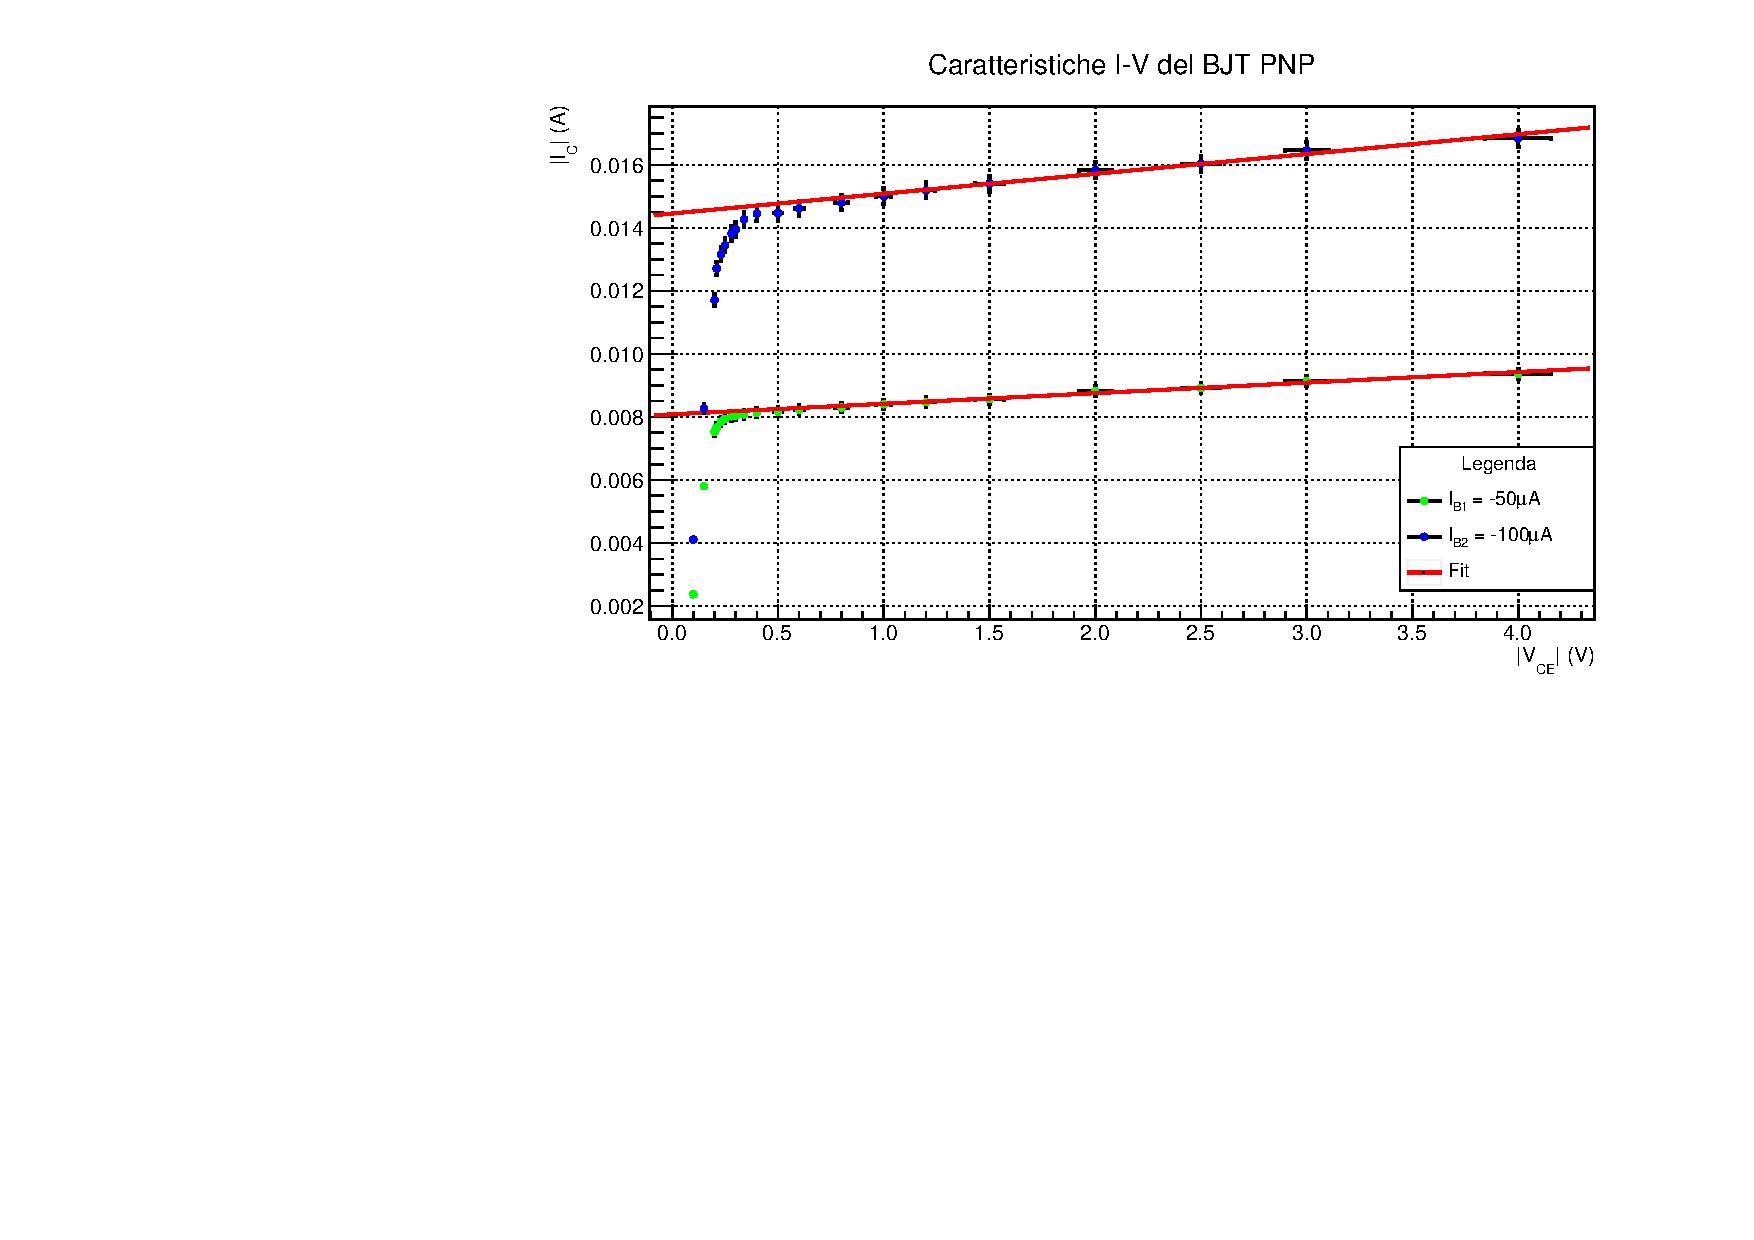
\includegraphics[width=0.9\textwidth]{image/fit.pdf}
    \caption{Grafico con relativi fit delle  caratteristiche $I_C$-$V_{CE}$. In verde riportiamo i dati relativi a $I_{B_1}$, mentre in blu quelli relativi a $I_{B_2}$. Per entrambi i casi il fit è stato svolto per valori della tensione $|V_{CE}|>1$ \si{V}.}
    \label{fig:fit}
\end{figure}

Con i dati riportati in \autoref{tab:data}, presente in \autoref{ch:data}, è stato possibile graficare gli andamenti $I_C$-$V_{CE}$ del transistor per le due correnti di base fissate $I_{B_1}$ e $I_{B_2}$. Per il calcolo delle incertezze sulle varie misure rimandiamo all’\autoref{ch:err}. Con le caratteristiche $I_C$-$V_{CE}$ del transistor è stato possibile effettuare un fit lineare pesato, secondo l'\autoref{eq:fit}, nella regione attiva per ciascun valore di $I_B$, come riportato in \autoref{fig:fit}.

Dopo aver estrapolato dai fit i valori di a e b per entrambe le caratteristiche, abbiamo ricavato la conduttanza $g$ e il guadagno $\beta$ a partire dalle relazioni \eqref{eq:conduttanza} e \eqref{eq:guadagno}. In particolare, per calcolare $\beta$ abbiamo fissato $V_{CE} = -1.0$ \si{V} come tensione di riferimento. Anche in questo caso, per il calcolo delle incertezze su $g$ e $\beta$ rimandiamo all’\autoref{ch:err}.  
Riportiamo i valori dei parametri trovati per le due differenti caratteristiche in \autoref{tab:fit_res}.

\begin{table}[htb]
    \centering
    \begin{tabular}{||c||c||c||}
    \hline \hline
    \multicolumn{3}{||c||}{\textsc{risultati dei fit}}\\
    \hline \hline
      & $I_{B_1} = -50$ \si{\micro\ampere} & $I_{B_1} = -100$ \si{\micro\ampere}\\
    \hline \hline
    $V_a$ & $(24 \pm 5)$ \si{V} & $(23 \pm 4)$ \si{V}\\
    $R_L$ & $(3.0 \pm 0.5)$ \si{\kilo\ohm} & $(1.6\pm 0.3)$ \si{\kilo\ohm} \\
    $g$ & $(0.33 \pm 0.06)$ \si{mS} & $(0.63 \pm 0.12)$ \si{mS} \\
    \hline
    $\beta$ & \multicolumn{2}{c||}{$(1.3 \pm 1.1) \cdot 10^{2}$} \\
    \hline\hline
    \end{tabular}
    \caption{Risultati dei fit con relativi valori della conduttanza $g$ e guadagno $\beta$.}
    \label{tab:fit_res}
\end{table}

\section*{Conclusione}
Per entrambi i valori della corrente di base $I_B$, la caratteristica $I_C$-$V_{CE}$ rispecchia l’andamento atteso: una rapida crescita iniziale, seguita da un tratto lineare nella regione attiva a pendenza non nulla tipico dell’effetto Early.

Le tensioni di Early misurate $V_{a_1}$ e $V_{a_2}$  sono tra loro compatibili come ci si aspettava. Inoltre, abbiamo un guadagno di corrente $\beta = (1.3 \pm 1.1) \cdot 10^{2}$ a prova del fatto che il transistor BJT PNP in configurazione a emettitore comune si comporta come un amplificatore di corrente. Infine, i valori di $R_L$ ottenuti dai fit rientrano nell'ordine di grandezza del \si{\kilo\ohm}, come previsto.

Notiamo inoltre che l’incertezza sul fattore di guadagno è molto alta, probabilmente per il basso grado di risoluzione del multimetro digitale usato durante l’esperienza.

\newpage
\section*{\Huge Appendice}
\appendix

\section{Dati raccolti} \label{ch:data}
\noindent I valori misurati delle correnti di base misurati sono $I_{B_1} = -(0.05 \pm 0.02)$ \si{\milli\ampere} e $I_{B_2} = -(0.10 \pm 0.02)$ \si{\milli\ampere}. I dati misurati relativi alle caratteristiche $I_C$-$V_{CE}$ sono riportati in \autoref{tab:data}. 
\begin{table}[htb]
    \centering
    \begin{tabular}{||c|c||c|c||c|c||}
        \hline \hline
        \multicolumn{6}{||c||}{\textsc{caratteristiche i-v in uscita}} \\
        \hline \hline
         & & \multicolumn{2}{c||}{$I_{B_1} = -50$ \si{\micro\ampere}} & \multicolumn{2}{c||}{$I_{B_2} = -100$ \si{\micro\ampere}}\\
         \hline
        $|V_{CE}|$ (\si{V}) & f.s. & $|I_{C_1}|$ (\si{\milli\ampere}) & f.s. & $|I_{C_2}|$ (\si{\milli\ampere}) & f.s.\\ \hline
        \csvreader[
            head to column names,
            separator=tab,
            % table head = $V_\text{MM}$ & f.s. & $V_\text{osc}$ & f.s.\\\hline
             late after line=\\
            % table foot = \hline \hline
            % table head = \toprule
        ]{data/data.csv}{}
        {\Volt  $\text{ }\pm$ \VoltErr & \VoltFs & \FCurr  $\text{ }\pm$ \FCurrErr & \CurrFs & \HCurr  $\text{ }\pm$ \HCurrErr & \CurrFs}\hline\hline
    \end{tabular}
    \caption{Dati relativi alle caratteristiche in uscita del BJT per due differenti correnti di base $I_{B_1} = -50$  \si{\micro\ampere} e $I_{B_2} = -100$ \si{\micro\ampere}.}
    \label{tab:data}
\end{table}

\section{Valutazione delle incertezze} \label{ch:err}
\subsection{Oscilloscopio}
Per calcolare l’incertezza $\sigma_V$ associata ad ogni singola misura di tensione $V$ effettuata con l’oscilloscopio, abbiamo utilizzato la formula: 
\begin{equation*}
    \sigma_V = \sqrt{{\sigma_L}^2 + {\sigma_Z}^2 + {\sigma_C}^2 }
\end{equation*}
con $\sigma_C = V \cdot \alpha$, dove $\alpha$ è la precisione dichiarata dal costruttore (che in questo caso è 3\%), mentre $\sigma_L$ e $\sigma_Z$ rappresentano rispettivamente l’errore sulla lettura e l’errore sullo zero, entrambi da determinare secondo la seguente relazione:
\begin{equation*}
    \sigma_L = \sigma_Z = \dfrac{V_\text{f.s.}}{5} \cdot N_\text{t.a.}
\end{equation*}
in cui $V_\text{f.s.}$ rappresenta il fondoscala utilizzato per la singola misura e $N_\text{t.a.}$ indica il numero di tacchette apprezzabili.

\subsection{Multimetro}
Per quanto riguarda l'incertezza $\sigma$ da associare ad ogni misura effettuata con il multimetro digitale, sono state sfruttate le specifiche riportate in \autoref{tab:multimetro}; dunque ad ogni misura $x$ bisogna associare un'incertezza $\sigma_x$ secondo l'espressione
\begin{equation*}
    \sigma_x = x \cdot \text{prec.} + \text{risoluzione} \cdot \text{digits} 
\end{equation*}
con $\text{prec.}$, $\text{risoluzione}$ e $\text{digits}$ da estrapolare dalle colonne in \autoref{tab:multimetro}.

% bisogna includere di section alternativo perché hyperref non riesce a leggere le cose in math mode
\subsection[Incertezze di g e di beta]{Incertezze di $g$ e di $\beta$}
Per stimare l'incertezza associata alle misure di $g$ e $\beta$ sono state usate le seguenti formule:
\begin{equation*}
    \Delta g = \dfrac{\Delta R_L}{{R_L}^2}
\end{equation*}
\begin{equation*}
    \Delta\beta = \left(\dfrac{\Delta I_{C_2} + \Delta I_{C_1}}{ I_{C_2} - I_{C_1}} + \dfrac{\Delta I_{B_2} + \Delta I_{B_1}}{ I_{B_2} - I_{B_1}}\right)
\end{equation*} 


\end{document}